\chapter{DigitClassifier tool}
	\label{chap:4_digitclassifier}
		This JdeRobot component (\autoref{sec:3_digitclassifier_jderobot}) was used on this project to land on the concept of neural networks.\\
	
		Its design aims to \textit{classify handwritten numbers} with the use of a Convolutional Neural Network (\autoref{sec:1_cnn}), which classifies the incoming images from a video source.\\
		
		\begin{figure}[h]
			\centering
			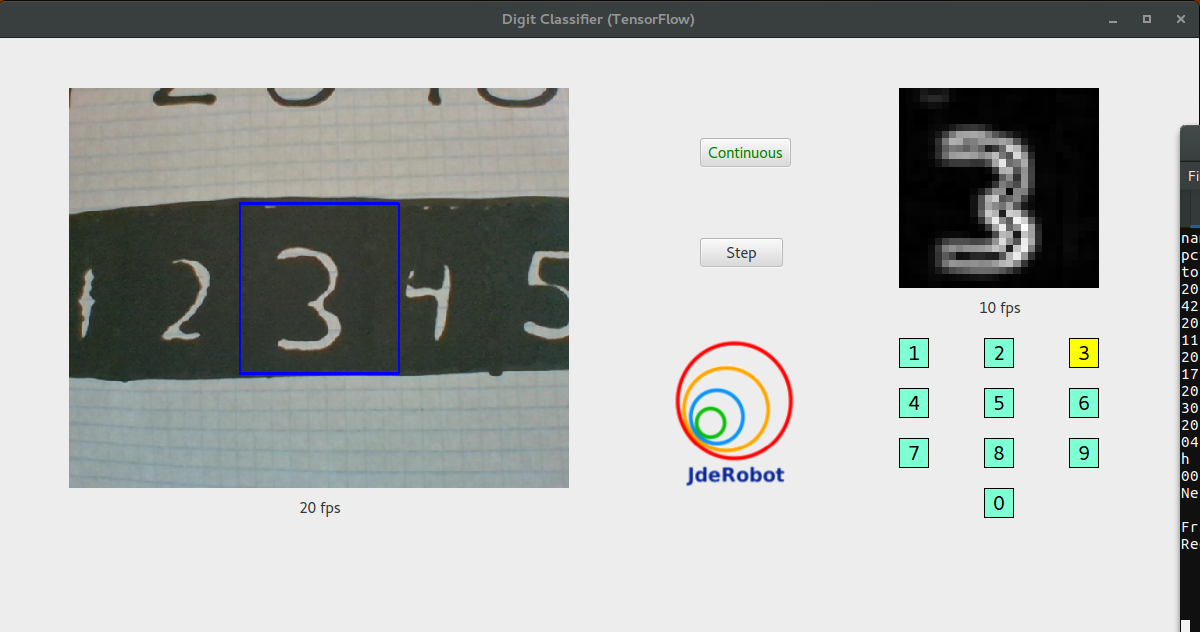
\includegraphics[width=4in]{images/digitclassifier}
			\caption{\texttt{DigitClassifier} on action.}
			\label{fig:4_digitclassifier}
		\end{figure}
		
		This kind of application (handwritten digits classification) is the typical first milestone to achieve in the domain of deep learning concepts and neural networks architectures, so lots of documentation are available online (a basic domain of the framework can be successfully achieved on the official TensorFlow tutorials\footnote{\url{https://www.tensorflow.org/tutorials/layers}} which, as said, teach how to deploy a handwritten digit classification system).\\


		As we mentioned, previous existing implementations were written in Keras \cite{dpascualhe} and Caffe \cite{noyaga} (Python libraries to implement Deep Learning algorithms), so we made the same on TensorFlow (\autoref{sec:3_tensorflow}), to accomplish an initial domain of this Machine Learning framework\footnote{Demonstration videos available on the MediaWiki page (\url{https://jderobot.org/Naxvm-tfg}).}.\\
		
		After this, Keras and TensorFlow versions were merged on a single JdeRobot component: \texttt{dl-digitclassifier}\footnote{\url{https://github.com/JdeRobot/dl-digitclassifier}}, which has the scope to be functional on both libraries and, in addition, supports image streams from ICE endpoints or ROS topics (thanks to the \texttt{comm} library).\\
		
		As it can be seen it the \emph{README} file\footnote{\url{https://github.com/JdeRobot/dl-digitclassifier/blob/master/README.md}} in the repository, configuring the component is made pretty simple thanks to the YML file, so the reader is asked to feel encouraged to give it a try.\\
		
	\section{Tool architecture}
		As specified in the requirements (\autoref{sec:2_requirements}), we divide the entire node functionality into individual tasks. These tasks have been implemented invoking a dedicated thread (using the \texttt{threading} library) for each one.\\
		
		\begin{figure}[h]
			\centering
			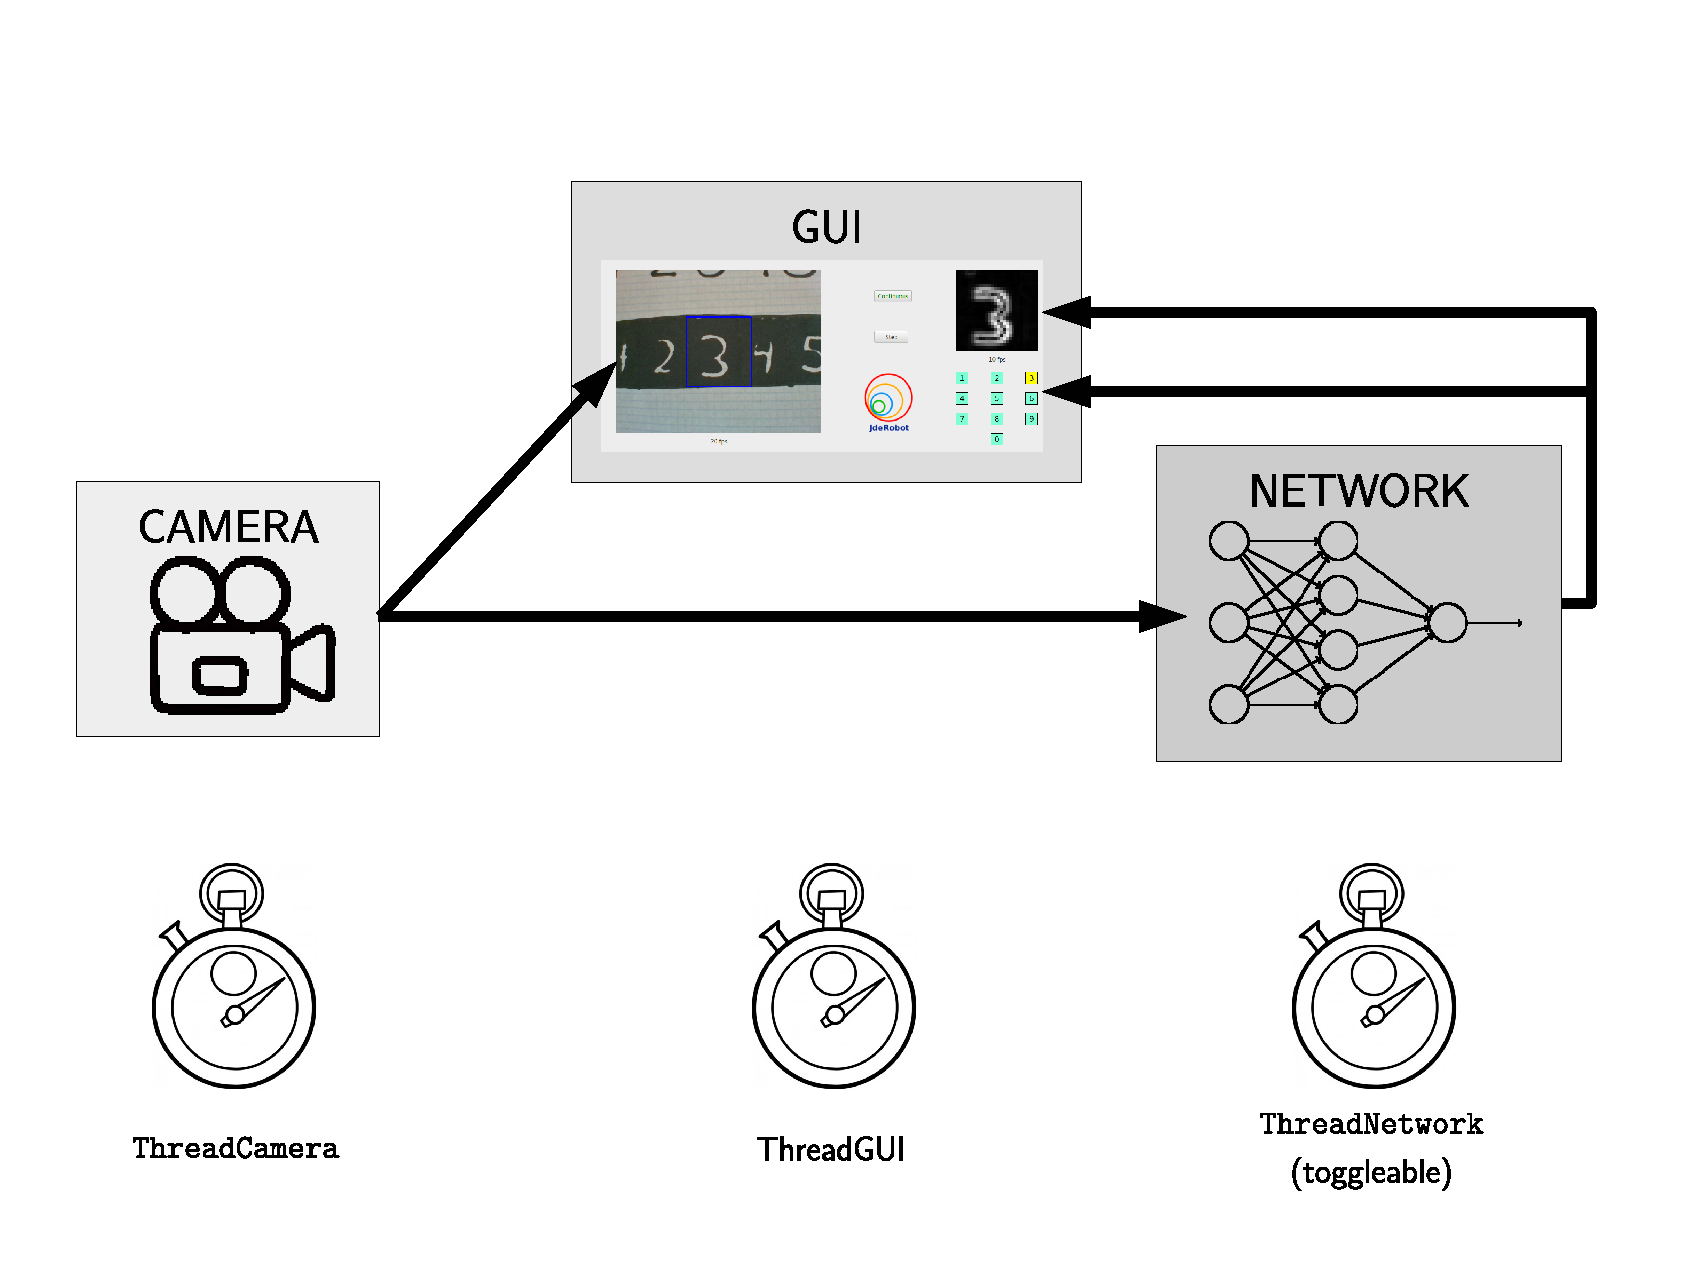
\includegraphics[width=5in]{images/digitclassifier_infrastructure}
			\caption{Infrastructure of the component (3 threads).}
			\label{fig:4_digitclassifier_infrastructure}
		\end{figure}
		
		
		
		This establishes the first functional difference with the previous version, which was powered by only 2 threads (for the camera and the GUI), performing on-demand (blocking) inferences on the neural network. Implementing a new thread dedicated to the neural network allows to have an instantaneous output digit from the network, ready to be easily grabbed. Nevertheless, care has to be put on respecting parallelism between threads. This infrastructure is optimum for asynchronism, which means that one component does not depend on any others (e.g. the GUI component does not need the network to finish the next inference and return the classified digit in order to refresh the interface: it grabs the last inference made by the network \emph{from the own network}, which will be automatically updated when a newer one is available). This implies a respect to the independence between threads. It is the key for an asynchronous behavioral, as we want the component to yield the best possible performance.\\
		
		
		Using the specified \texttt{threading} library, this deployment is as easy as making a custom definition of the \texttt{\_\_init\_\_()} and \texttt{run()} methods:
		
		
		\begin{lstlisting}
...
import threading
from datetime import datetime
...

class MyThread(threading.Thread):

	def __init__(self, foo, bar):
		'''
		This is the method which will be called at the creation of the thread.
		'''
		self.my_foo = foo
		self.my_bar = bar
		self.time_cycle = 100 # ms
		threading.Thread.__init__(self)  # Rest of the initialization.
	
	
	def run(self):
		'''
		This is the task the thread will perform once.
		If we put an infinite loop inside, we have a periodic thread.
		'''
		while True:
		start_time = datetime.now()
		# Grab an image, or run an inference on the neural network...
		self.my_foo.doMyStuff(self.my_bar)
		end_time = datetime.now()
		dt = end_time - start_time
		
		# If it did not take the refresh time, it sleeps until it arrives.
		if dt < self.t_cycle:
		sleep(self.t_cycle - dt)
		
		\end{lstlisting}
		
		So, we can create versions of this generic class, and then instantiate them, as performed on \autoref{fig:4_digitclassifier_code}. This way, we have already created and started the parallel threads performing their own tasks on an asynchronous way. In addition, it is possible to control the update period of the thread, so we can decide how much time it will be elapsed between two consecutive executions of the task (and of course this is a tunable parameter).
		
		\begin{figure}[h!]
			\centering

			\begin{lstlisting}
import Camera, ThreadCamera
import GUI, ThreadGUI
import Network, ThreadNetwork
...


# We instantiate each object with its pertinent thread...
cam = Camera(cam_parameters)
t_cam = ThreadCamera(cam)

gui = GUI(gui_parameters)
t_gui = ThreadGUI(gui)

net = Network(net_parameters)
t_net = ThreadNetwork(net)

# Communicate them (according to the scheme)...
net.setCamera(cam)
gui.setCamera(cam)
gui.setNetwork(network)

# And start the application!
t_cam.start()
t_gui.start()
t_net.start()

gui.show()

	
			\end{lstlisting}
			
			\caption{Schematic code to instantiate the components of the node.}
			\label{fig:4_digitclassifier_code}
		\end{figure}

		
	\section{Image processing}
		For every digit recognition system using a CNN, the approach is the same: \emph{processing a 28$\times$28 px image}\footnote{This particular shape is due to the used dataset, as it will be seen later.} containing a binary image of the digit itself. In addition to this, our system aims to a robust and correct classification at every feasible situation. Handwritten digits can often be found in visually harsh environments (poor quality sensor or lighting, trace indistinguishable of the background, etc.). Given this, before inserting an image on the network, we have to subject it to a \emph{preprocessing} pipeline:
		
		\begin{enumerate}
			\item Grab the central region of the incoming image from the camera (blue square on \autoref{fig:4_digitclassifier}).
			
			\item Convert the image to grayscale, as the color information is not relevant (hence, the network does not deal with RGB images, but just a grayscale 28$\times$28 matrix).
			
			\item Soften the image with a \emph{gaussian blur}, in order to reduce the possible noise on the image. We convolve the image with a square kernel of size 5 px.
			
			\item Resize the image to the necessary shape of 28$\times$28 pixels.
			
			\item Lastly, we \emph{extract the edges} of the image. This is not trivial, as the information we want to observe for the digits are the \emph{edges}. Otherwise, images on different contrast conditions would not be supported, as that would imply very different weights on the network for each situation. For this edge extraction, we apply a Sobel operator (which can be seen like computing the directional gradient/derivative in the image, as stated in \cite{sobel}) on each direction (vertical/horizontal), in order to detect the existing edges, and add them together in a single edge image, which is the final output of the pipeline.
		\end{enumerate}
		
		As a result, we obtain a softened shape map (even from different images, as seen on \autoref{fig:4_preprocessing}), which is a good start for the neural network to infer. This image is  shown in the GUI. This pipeline will be applied to every image (in the training process and while performing a new inference).
		
		\begin{figure}[h]
			\centering
			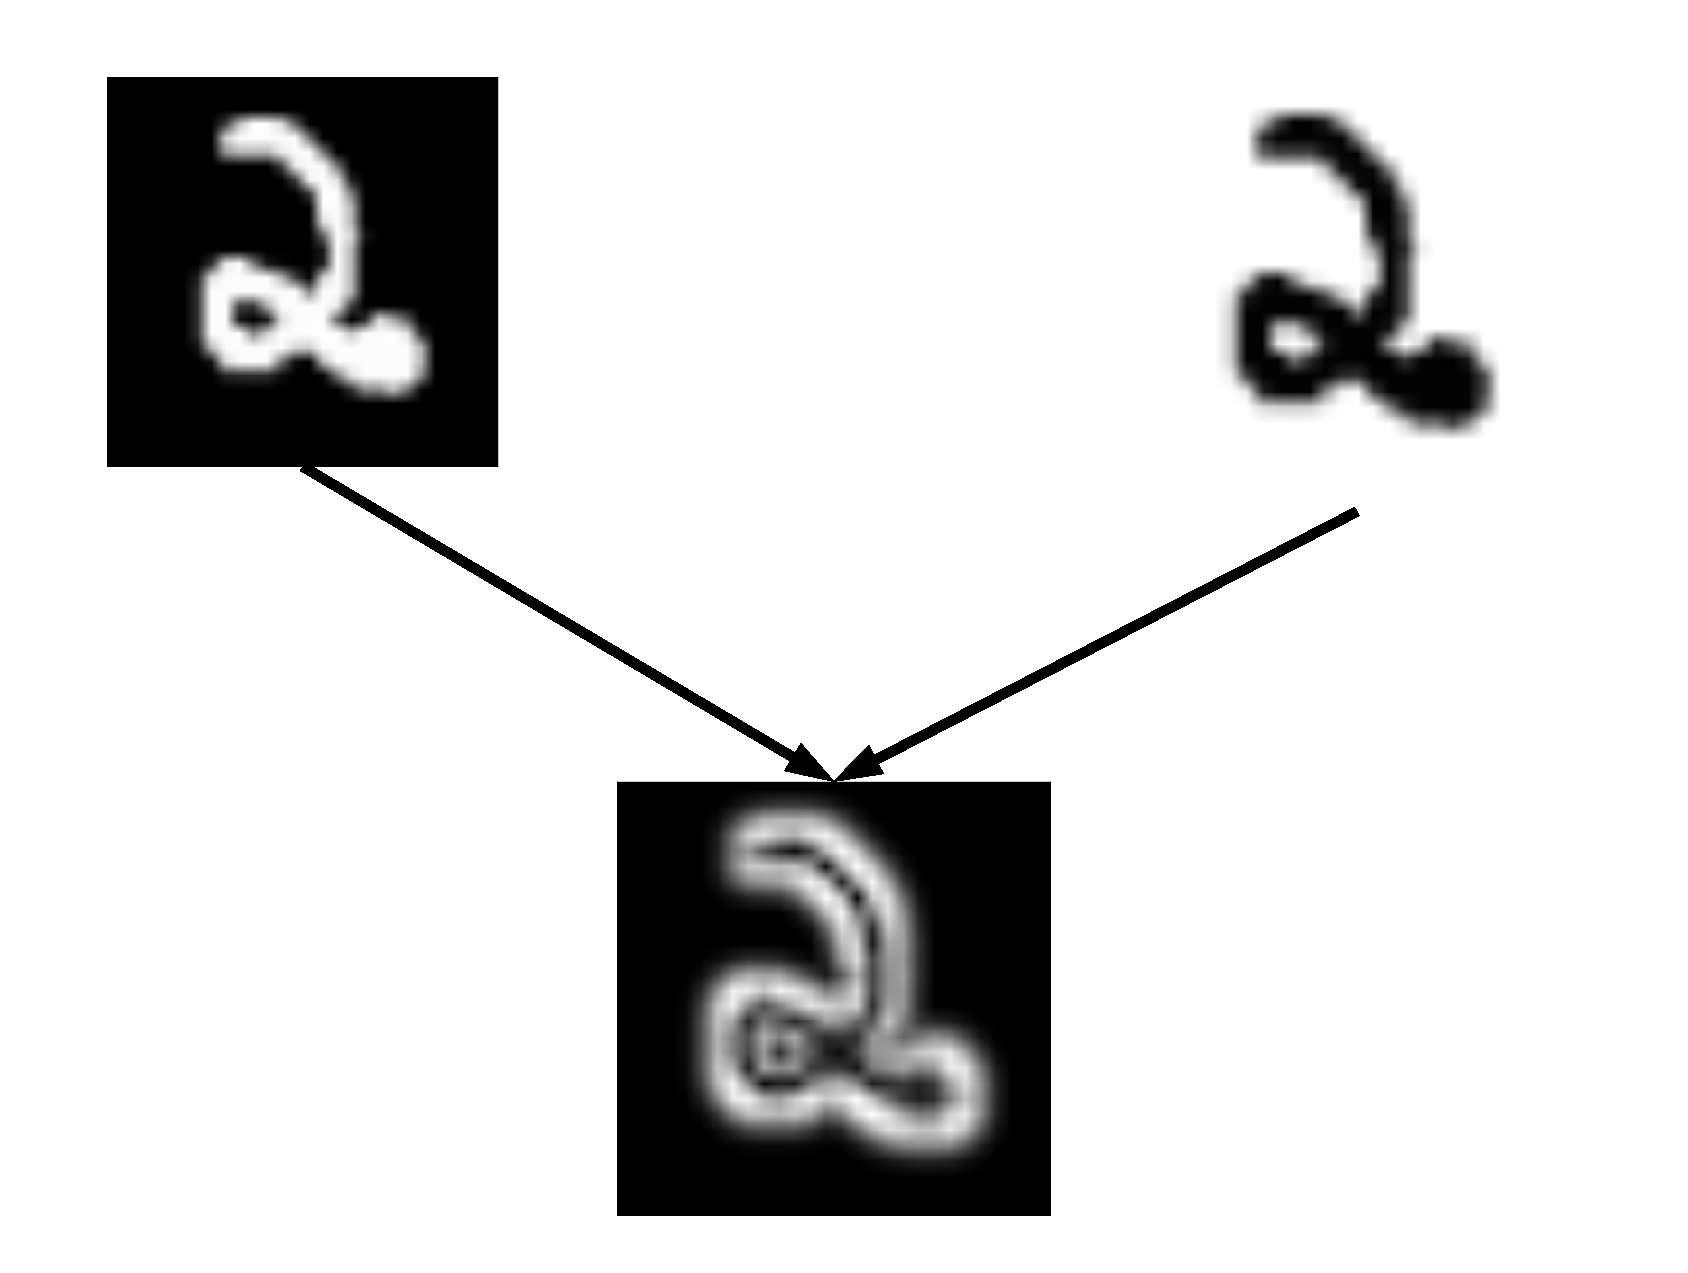
\includegraphics[width=5in]{images/digits_preprocessing}
			\caption{Result of the preprocessing (identical for both images).}
			\label{fig:4_preprocessing}
		\end{figure}

	\section{Digit classification CNN}
		\label{sec:4_classif_cnn}
		The implementation of this convolutional neural network consists of a concatenation of layers, following the schema shown on \autoref{fig:4_digitclassifier_neural_structure}. These layers are disposed in a serial structure, so the output of one layer (a vector containing what each neural activation function yields) acts as the input for the next one.
		
		For this reason, we need a first input layer, where all the pixels of the input image are mapped to a input neuron, on a bijective way.\\
		
		As stated before, the input shape for the images is 28$\times$28 px (a total of $28^2 = 784$ px), so we firstly perform a \emph{reshape} operation, which arranges the pixels on a 1-dimensional array of pixels. That will be the input for the network.
		
		\begin{figure}[h]
			\centering
			\begin{subfigure}[h]{0.65\linewidth}
				\centering
				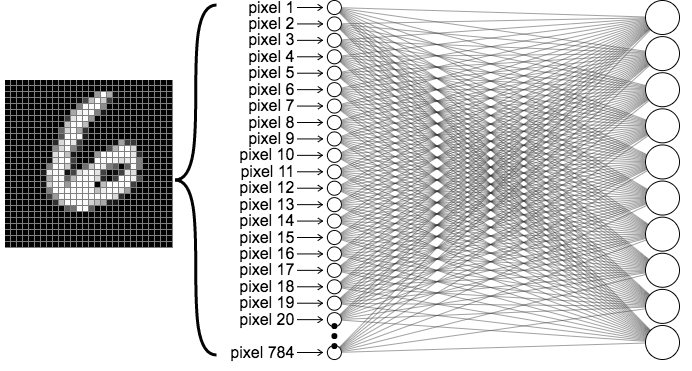
\includegraphics[width=4in]{images/mnist_net_example}
				\caption{High level layers visualization.}
			\end{subfigure}
			\begin{subfigure}[h]{0.3\linewidth}
				\centering
				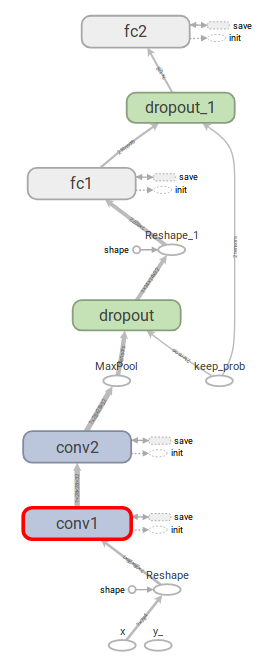
\includegraphics[width=1.7in]{images/digitclassifier_network_graph}
				\caption{Low level layers visualization.}
			\end{subfigure}
			\caption{Model of the implemented CNN for our system.}
			\label{fig:4_digitclassifier_neural_structure}
		\end{figure}
		
		\begin{enumerate}
			\item \texttt{conv1}: first convolutional layer. As described in \autoref{sec:1_cnn}, it performs a 2D convolution between a $5px \times 5px$ square mask/kernel (\texttt{W\_conv1}), and the image (which is seen again as a $28 \times 28$ matrix to perform the convolution). Later, the layer adds a bias/intercept term (\texttt{b\_conv1}). Thus, we obtain the activation for each neuron (the ReLU operator applied to the local convolution in the environment of that particular pixel), \texttt{h\_conv1}.
			
			\begin{lstlisting}
# Illustrative purposes.
# Some additional parameters (padding, stride) ignored.
h_conv1 = tf.nn.relu(tf.nn.conv2d(x, w_conv1) +  b_conv1)
			\end{lstlisting}
			
			To get a better understanding of what is happening here, we can have a glance of the weights learned on each neuron, for each digit (as we will study further below), on the \autoref{fig:4_activation_maps}.
			
			\begin{figure}[h]
				\centering
				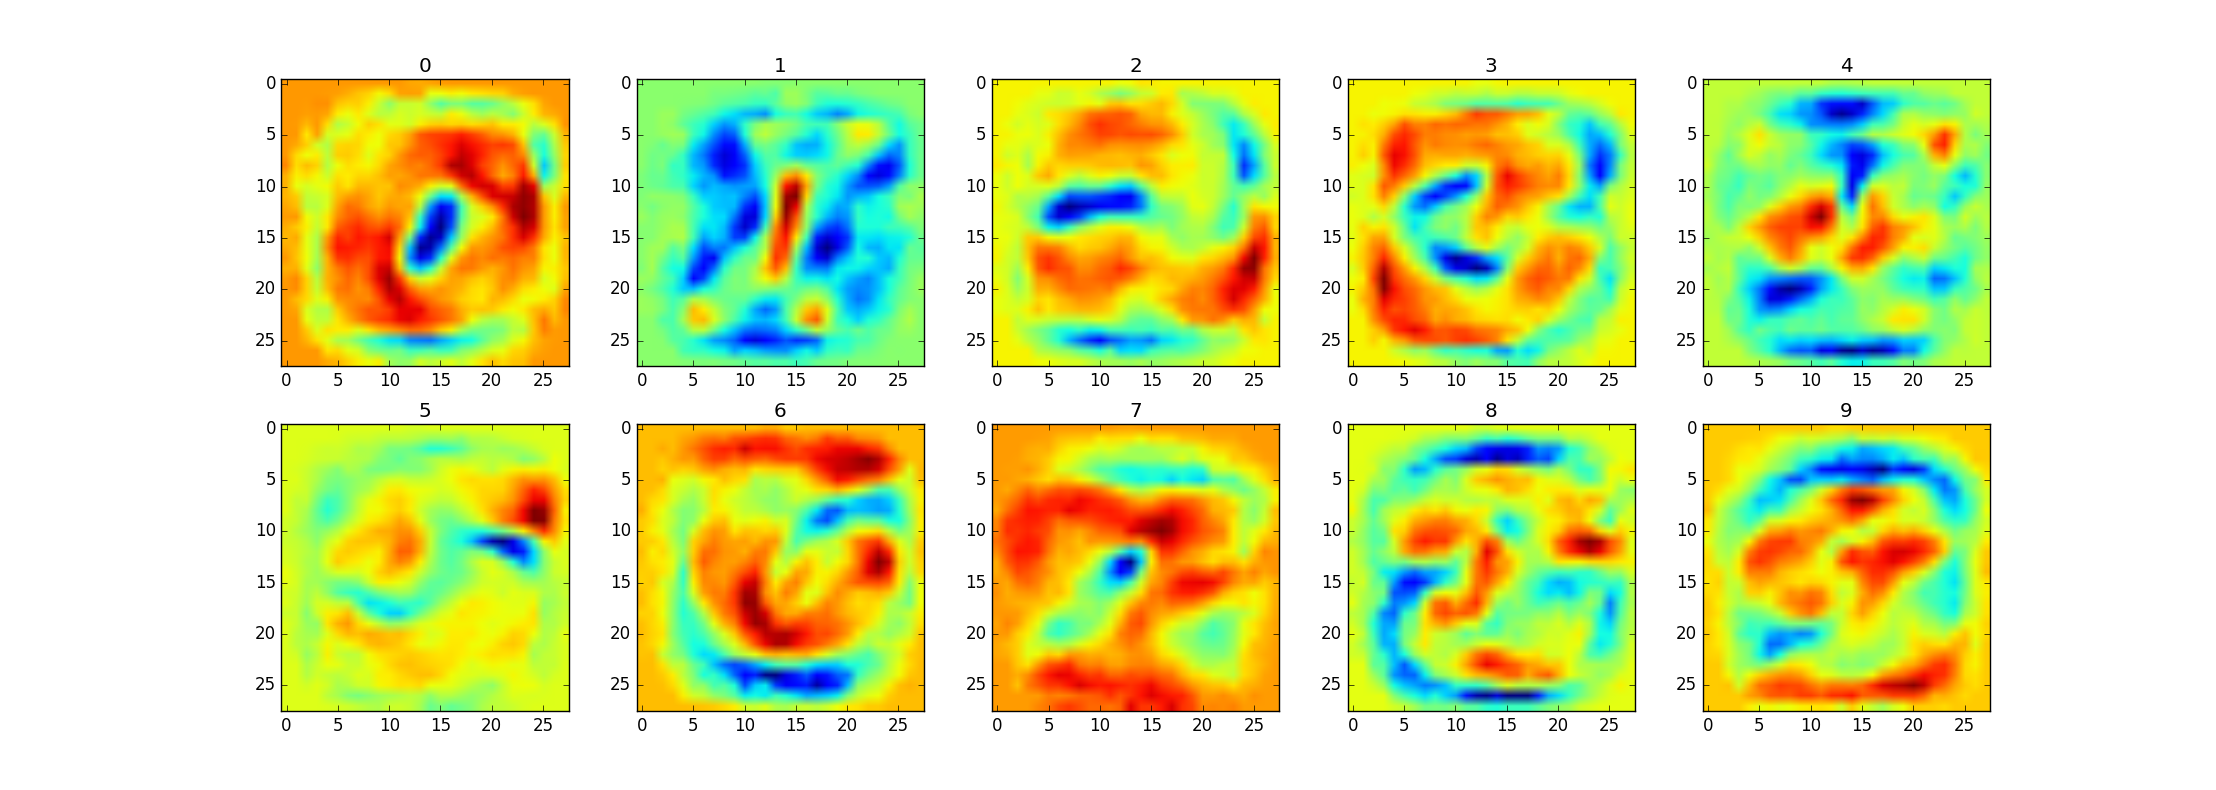
\includegraphics[width=6in]{images/digitclassifier_activation_maps}
				\caption{Heatmap for the learned weigths for each pixel and labeled digit.}
				\label{fig:4_activation_maps}
			\end{figure}
			
			This can begin to illustrate what is happening here: each neuron has a set of 10 tunable kernels, which depend on the value of what it has seen during the training process on its corresponding pixel and its environment. This illustration belongs to a simplified version of the network, where a convolution is not performed, but a simple \emph{matrix multiplication} (which can be seen as a convolution of kernel size equal to 1). So, we can see that the network is just learning where typically enabled pixels are situated on the input for each possible label ($0-9$).
			
			
			\item \texttt{conv2}: second convolutional layer. It performs the same operation taking the output from the previous layer as an input, using a different weights mask and bias terms.
			
			\begin{lstlisting}
h_conv2 = tf.nn.relu(tf.nn.conv2d(h_conv1, w_conv2) + b_conv2)
			\end{lstlisting}
			As we stated before, the tensor which will be convolved with the weights of this layer (\texttt{w\_conv2}) is now the output of the previous layer (\texttt{h\_conv1}).\\
			
			So far, what we have done is extracting patterns on each digit type (e.g. discovering typical circles on $0$ and $8$, which are always present on the same zone of the image).\\
			
			\item \texttt{pooling}: as the activation maps can be growing in size as we perform feed forward propagation, a \emph{pooling} operation is performed. It consists of spatially downsampling its input (the previous layer activation map). Concretely, we retain the \textit{maximum} value for each 2 pixels, which is known as \texttt{2x2 max pooling} (\autoref{fig:4_max_pooling}).
			
			\begin{figure}[h]
				\centering
				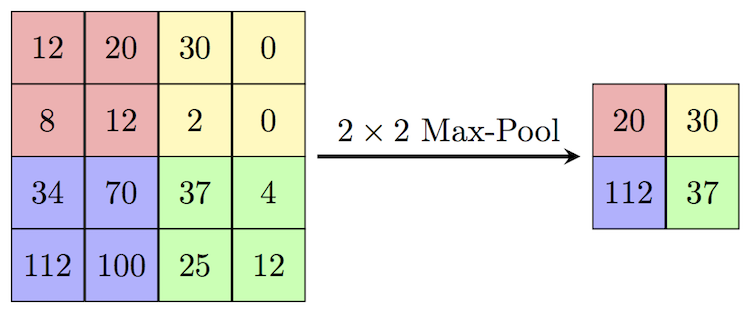
\includegraphics[width=4in]{images/max_pool}
				\caption{Max-pooling operation on a matrix.}
				\label{fig:4_max_pooling}
			\end{figure}
			
			\begin{lstlisting}
# Some additional parameters ignored here
# (kernel size, strides, padding).
h_pool = tf.nn.max_pool(h_conv2)
			\end{lstlisting}
			
			\item \texttt{dropout}: this layer does not strictly perform any mathematical operations. It lets pass the tensors through it, but randomly switching off some neurons. This is parameterized by a user input, using a variable called \texttt{keep\_prob} (which stands for the probability of a neuron staying switched on). In our case, we set it to $0.5 \ (50\%)$ during the training process, to avoid overfitting by forcing the network to modify the neural paths randomly, as not every neuron is available on every moment. This is kind of similar to augmenting the dataset during the training process. The rest of the time (when the network is used to make inferences), this parameter is set to $1.0 \ (100\%)$, which means that no neurons are switched off at all.\\
			
			\begin{lstlisting}
# The value for keep_prob is parameterized.
h_drop1 = tf.nn.dropout(h_pool, keep_prob)
			\end{lstlisting}
			
			
			\item \texttt{fc1}: first fully connected layer. So far, we have seen the pipeline as operable matrices. From now on, we go back to the \emph{single-dimension} activation map (array of outputs) model.
			
			These layers, also known as \emph{dense} layers, are distinguised because every neuron is connected to every activation from the previous layer. So, this kind of layers are used for \textit{pattern association with labels}, due to the relationship they can infer between every input.\\
			
			A thumb rule on this kind of layers is the more neurons included, the better generalization (the more correlation patterns we can detect between the activated zones on the incoming activation map). So, our implementation establishes a first dense layer of $14 \cdot 14 \cdot 32 = 6272$ neurons.\\
			
			\begin{lstlisting}
# Firstly, the last activation map is flattened into a 1 dimension array.
h_pool_flat = tf.reshape(h_drop1, [-1, 14*14*32])

# We model the full connection as a matricial multiplication
# (with a weight size of 14*14*32)
h_fc1 = tf.nn.relu(tf.matmul(h_pool_flat, w_fc1) + b_fc1)
			\end{lstlisting}
			
			\item \texttt{dropout}: to gain in strength, we deploy another dropout layer (which switches off random neurons with the same probability than the first dropout layer). This is remarkable, as we had performed a dropout process on the \textit{feature retrieval phase (first layers)}, but not on the \textit{pattern searching phase (dense layers)}.
			
			\begin{lstlisting}
h_drop2 = tf.nn.dropout(h_fc1, keep_prob)
			\end{lstlisting}		

			\item \texttt{fc2}: the output layer. It connects all the outputs of the previous dense layer and groups the output in a 10-dimensional vector, which contains the obtained \emph{logits}, a representative number for that class on the given image, which can be interpreted as a linear \emph{reward/tendence} \cite{sutton-barto} to belong to that class.
			
			As the last step, it applies a \textit{softmax} ($\sigma$) function to the output:
			\begin{equation}
				\sigma(z)_j = \frac{e^{z_j}}{\sum_{k=1}^{K}e^{z_k}}
			\end{equation}
			This function normalizes the output, mapping it between 0 and 1. This converts the mentioned raw numerical output into a \emph{probability} of being the given class (where the sum of the probability of all possible classes converges to $1$).
			
			\begin{lstlisting}
class_tendences = tf.nn.relu(tf.matmul(h_drop2, w_fc2) + b_fc2)

# Output (this is the called node to get the total inference output):
y = tf.nn.softmax(class_tendences)
			\end{lstlisting}
			
		\end{enumerate}
		
		This way, the total output of the CNN is a vector containing the probability of the image belonging to each class. If we keep the argument(s) of the maxima (\texttt{argmax}), we can find the most suitable class for that image.\\
		
		At this point, we can remember that the images entering into the network have been preprocessing, looking for the edges, so the learning process and the weights used through all the recently described pipeline can be generalized to all kind of images (as we will pass it previously through the Sobel edge detection filter).\\
			

		\subsection{Training the network}
		\label{sec:4_train}
			The reviewed pipeline is performed on an image, since it enters on the neural network until it goes out, passing through all the defined layers performing what is called \emph{feed-forward} propagation. However, the values of the activation maps and, hence, of the dense layer outputs (which determine the resulting class) depend on a relatively huge number of neurons, each one with its own weights and biases (for each class). As we can see, that is a ridiculous number of parameters to tune manually, hence we tune it automatically performing what is called \emph{backpropagation}.\\
			
			This backpropagation algorithm \cite{Rumelhart1986} performs a standard feedforward propagation (as described before) on what we call \emph{training set} (labeled images that will be used \emph{exclusively} for this purpose), which the system takes as examples which to learn of. Then, it compares the obtained output class ($argmax(softmax())$) for each input, and adjusts all the weights of the network, seeking to ensure that the difference between the \emph{desired} output (the \emph{ground truth} labels) and the \emph{obtained} result is minimum. This difference is computed and represented by a value which we call \emph{loss/cost} (the higher its value is, the worse, as there is a bigger difference between the correct and the obtained output).\\
			
			This tuning process is performed using what is called an \emph{optimizer}, which is an algorithm to search the optimum direction and magnitude update for every weight present on the network, depending on the obtained differences. As this can be such a complex process, it is performed on an \emph{iterative} way: evaluate a batch\footnote{A \emph{batch is a set of examples, which are introduced to the network on a stacked way.}} of training images, obtain the value for its loss, compute the suitable update values, and perform the weights update (scaled by what is called \emph{learning rate}, which determines the magnitude of the leap for each update). This way, after a number of iterations\footnote{This necessary number can not be determined, as it depends hugely on the dataset, purpose, network structure, learning parameters, etc. The best option is to monitor the loss/accuracy values during the training process, and stop it when these values converge (otherwise it could result in \emph{overfitting}, that is not convenient as it will only work fine on already seen examples).}, the model should converge to a global minimum for the loss function, which hopefully means that a suitable value for each weight has been found. This is the mechanism responsible of fitting the weights, so thank to it, we obtained, among many others, a reasonable values for the input layer on this network (\autoref{fig:4_activation_maps}).\\
			
			On our application, the chosen function to compute the lost value is the \emph{softmax cross-entropy} (as the name indicates, it is based on the \emph{softmax} version of the output, which means that it works with probabilities). It stands for the difference between the correct probability for a particular class (remember that each class is represented by a neural unit on the output layer: 1 if it's the suitable class, 0 otherwise), and the obtained output \emph{probability} \cite{cross-entropy}.
			
			This value is obtained on this way, being $y$ the binary correct output, and $p$ the computed softmaxed probability:\\
			
			\begin{equation}
				-(y \cdot log(p)) + (1-y) \cdot log(1-p)
			\end{equation}
		
			With respect to the optimization algorithm, the most intuitive option is the \emph{gradient descent algorithm} (that, in fact, is perfectly implementable on this system). Instead, we use the \emph{Adam} algorithm, which is an extension of the gradient descent approach. Its advantage is that it \emph{automatically adapts the learning rate} of the parameters adjustment, by computing its moving averages and variances (\emph{momentums}) \cite{adam-optimizer}. This is some more computationally expensive, but it is affordable. In exchange, we obtain an automatic training hyperparameters tuning, which is reflected in a faster and finer convergence to a correct value. It takes as input the cost function, and struggles to iteratively minimize it.\\
			
			
			Putting all this together, we can build these nodes on TensorFlow on an easy way, gearing the output (\texttt{y}) to the new optimization blocks:
			
			\begin{lstlisting}
# Cost function:
cross_entropy = tf.reduce_mean(
                  tf.nn.softmax_cross_entropy_with_logits_v2(labels=self.y_,
                                                                  logits=self.y))


# Optimizer (this is the called node during the training process):
train_step = tf.train.AdamOptimizer(1e-4).minimize(cross_entropy)

			\end{lstlisting}
		
		\subsection{MNIST dataset}
			\label{sec:4_mnist}
			MNIST (\emph{Modified National Institute of Standards and Technology database})\footnote{\url{http://yann.lecun.com/exdb/mnist/}} is a public database, which contains labeled binary images of handwritten digits. It is the result of jointing and shuffling\footnote{This is an important step to perform on databases, because we have to be sure of a correct \emph{generalization}: the data used for training must be of the same kind than for testing, to obtain fair results independently of the chosen dataset on each step.} two previous NIST's special databases (SD-1, containing digits written by Census Bureau employees, and SD-3, containing digits written by students), which were originally designed as training and test sets, respectively.\\
			
			All the included images respect the same format, with two key aspects:
			\begin{itemize}
				\item The images are \emph{square} $28 \times 28$ pixels matrices, containing the whole number (and anything else).
				
				\item The pixels represent binary values. This means that a pixel can only take values as \emph{digit} or as \emph{background}.
			\end{itemize}
			
			Given this, there are two image sets at our disposal: $60,000$ images for training, and $10,000$ images for testing\footnote{The \emph{test} set must not be used on the training process under any circumstance, to avoid unfair results, as this would be the equivalent to know an exam questions before taking it.}. Among all of them, we can obtain random examples (\autoref{fig:4_mnist_standard}).\\
			
			This is the image source we use to train our component, remembering that every image is preprocessed (\autoref{fig:4_preprocessing}) before going into the network.\\
			

		\subsection{Dataset augmentation}
			David Pascual \cite{dpascualhe} and Nuria Oyaga \cite{noyaga} performed what is called a \emph{data augmentation} over the MNIST dataset, with the objective of \emph{pretend} to have a bigger number of samples to train.\\
			
			It consists of taking the existing images (on the standard MNIST dataset) and apply to it random (although controlled) transformations: each image suffers \emph{translations, rotations and zooms}, in addition to \emph{gaussian noise}. This has a double purpose: to \emph{get a bigger number of samples} (which is always a good thing), and to \emph{make a better model to process real world images}. As this network will classify real incoming digits from a camera, these digits will have most probably suffered noise (because of the camera and light conditions) and various geometrical transformations (as it can be shown to the camera with a slight tilt, or on a different background, etc.). Thus, we need to create a neural network which is ready to deal these harsh conditions. That is the main reason to augment the dataset performing these transformations.\\
			
			Taking all this on account, we have at our disposal the datasets they created\footnote{A link to download them for future usages is available on the \emph{README} file of the repository:\\ \url{https://github.com/JdeRobot/dl-digitclassifier}.}. As we can see on \autoref{fig:4_mnist_augmented}, this set of images is much harsher than the standard one (\autoref{fig:4_mnist_standard}). This will allow to create a much more robust model to classify real world digit images.\\



			\begin{figure}[h!]
				\centering
				\begin{subfigure}[h]{0.4\linewidth}
					\centering
					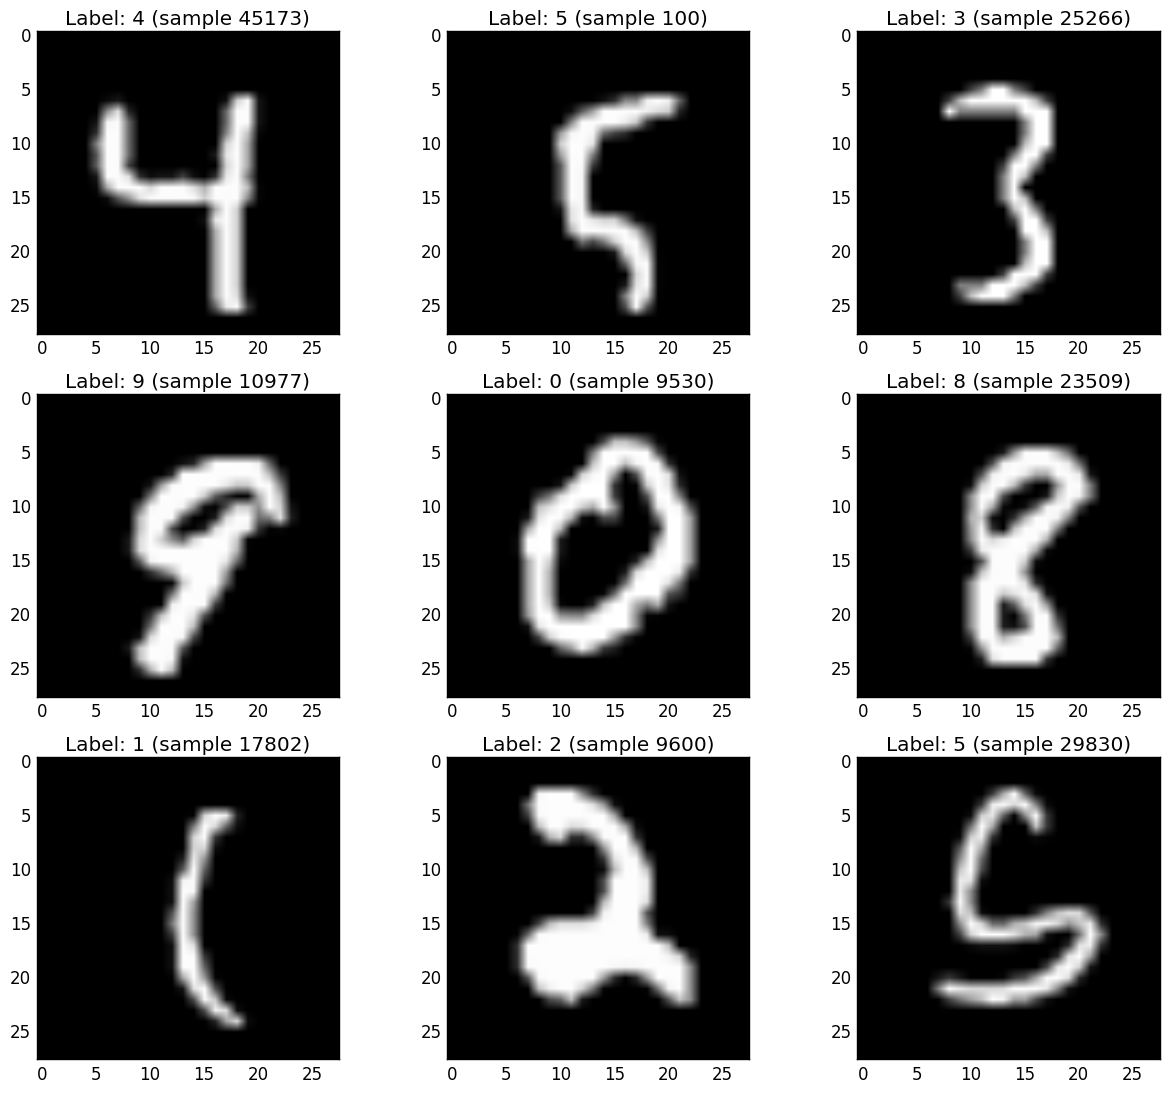
\includegraphics[width=2.3in]{images/training}
					\caption{Standard MNIST dataset.}
					\label{fig:4_mnist_standard}
				\end{subfigure}
				\qquad
				\begin{subfigure}[h]{0.45\linewidth}
					\centering
					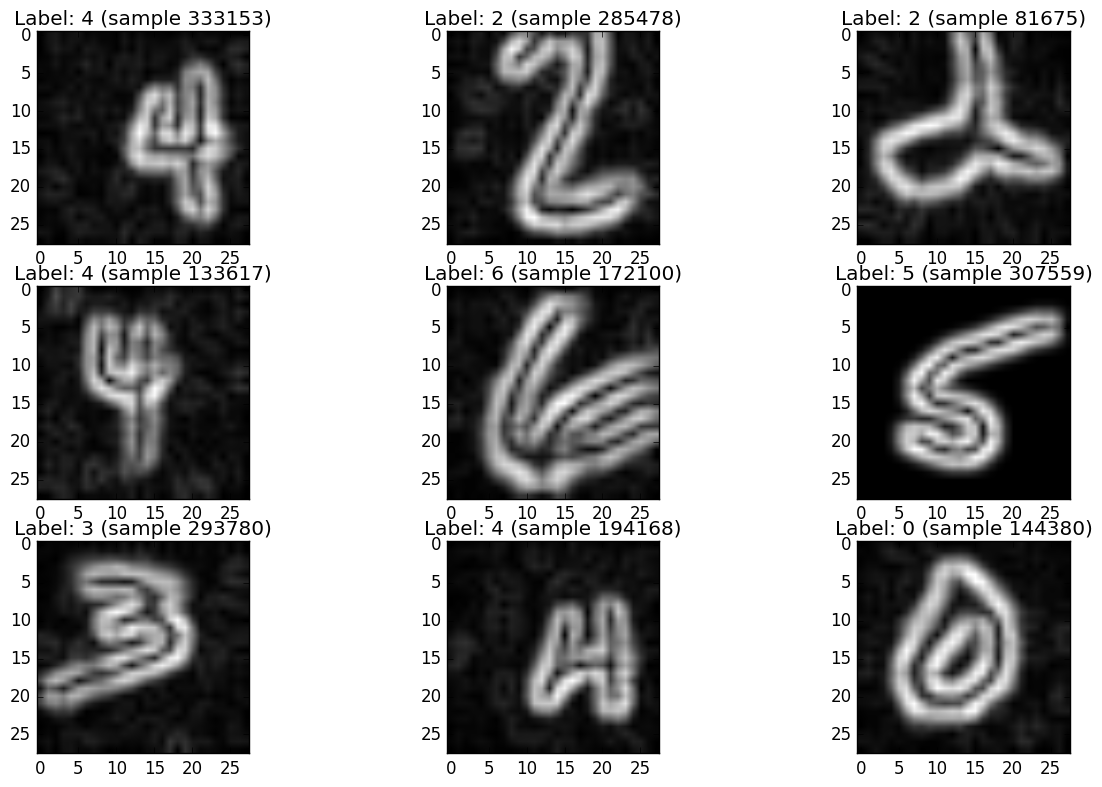
\includegraphics[width=3.2in]{images/training_augm}
					\caption{Augmented MNIST dataset.}
					\label{fig:4_mnist_augmented}
				\end{subfigure}
				\label{fig:4_mnist}
				\caption{Set of 9 random images extracted from the datasets.}
			\end{figure}


			These augmented datasets can be combined in different proportions (how many modified images are created for each standard image), which is typically indicated at its name: \texttt{training set x-y} means that there are \texttt{y} modified images for each \texttt{x} original one. To train the definitive model implemented on the classifier, we use the \texttt{1-6} model, which means that there are 6 modified versions of an image vs. 1 copy of the original one.

